\documentclass[conference,compsoc]{IEEEtran}
\IEEEoverridecommandlockouts
% The preceding line is only needed to identify funding in the first footnote. If that is unneeded, please comment it out.

\usepackage{cite,doi}
\usepackage{amsmath,amssymb,amsfonts}
\usepackage{algorithm,algpseudocode}
\usepackage{graphicx}
\usepackage{textcomp}
\usepackage{xcolor}
\usepackage{cleveref}
\usepackage{tikz}
\usepackage{mathtools}
\usepackage{ourmacros}
\def\BibTeX{{\rm B\kern-.05em{\sc i\kern-.025em b}\kern-.08em
    T\kern-.1667em\lower.7ex\hbox{E}\kern-.125emX}}

\newcommand{\LM}[1]{\textcolor{blue}{\textbf{Lawton}: #1}}    
\newcommand{\GB}[1]{\textcolor{red}{\textbf{Grey}: #1}}
\newcommand{\RK}[1]{\textcolor{blue}{\textbf{Ramki}: #1}}


\begin{document}

\title{Parallel Hierarchical Clustering using \\ Rank-Two Nonnegative Matrix Factorization
\thanks{This material is based upon work supported by the National Science Foundation under Grant No. OAC-1642385 and OAC-1642410.
This manuscript has been co-authored by UT-Battelle, LLC under Contract No. DE-AC05-00OR22725 with the U.S. Department of
Energy. This project was partially funded by the Laboratory Director's Research and Development fund. This research used resources
of the Oak Ridge Leadership Computing Facility at the Oak Ridge National Laboratory, which is supported by the Office of Science of
the U.S. Department of Energy.}
}

\author{\IEEEauthorblockN{Lawton Manning and Grey Ballard}
\IEEEauthorblockA{Wake Forest University \\
Winston-Salem, NC, USA \\
\{mannlg15,ballard\}@wfu.edu}
\and
\IEEEauthorblockN{Ramakrishnan Kannan}
\IEEEauthorblockA{Oak Ridge National Laboratory \\
Oak Ridge, TN, USA \\
kannanr@ornl.gov}
\and
\IEEEauthorblockN{Haesun Park}
\IEEEauthorblockA{Georgia Institute of Technology \\
Atlanta, GA, USA \\
hpark@cc.gatech.edu}
}

\maketitle

\begin{abstract}
Nonnegative Matrix Factorization (NMF) is an effective tool for clustering nonnegative data, either for computing a flat partitioning of a dataset or for determining a hierarchy of similarity.
In this paper, we propose a parallel algorithm for hierarchical clustering that uses a divide-and-conquer approach based on rank-two NMF to split a data set into two cohesive parts.
Not only does this approach uncover more structure in the data than a flat NMF clustering, but also rank-two NMF can be computed more quickly than for general ranks, providing comparable overall time to solution.
Furthermore, the rank-two NMF algorithm can be parallelized efficiently using a computational kernel similar to matrix-vector multiplication.
Our data distribution and parallelization strategies are designed to maintain computational load balance throughout the data-dependent hierarchy of computation while limiting interprocess communication, allowing the algorithm to scale to large dense and sparse data sets.
We demonstrate the scalability of our parallel algorithm in terms of data size and number of processors, and apply the hierarchical clustering approach to large (dense) hyperspectral imaging and (sparse) text document data.
\end{abstract}

%\begin{IEEEkeywords}
%component, formatting, style, styling, insert
%\end{IEEEkeywords}

\section{Introduction}

\GB{Prof Park, can you draft an introduction?  We are focusing on the dense case and using HSI and image clustering as applications.  Section 4 is still unfinished, but nearly all of the performance plots are there.  Feel free to leave placeholders for details that aren't obvious, we can clean them up Wednesday night.}

\section{Preliminaries and Related Work}
\label{sec:prelim}

\subsection{NMF}

The NMF constrained optimization problem
$$\min_{\M{W},\M{H}\geq \M{0}} \|\M{A} - \M{W}\M{H}^\Tra\|_2$$
is nonlinear and nonconvex, and various optimization techniques can be used to approximately solve it.
A popular approach is to use alternating optimization of the two factor matrices because each subproblem is a nonnegative least squares (NNLS) problem, which is convex and can be solved exactly.
Many block coordinate descent (BCD) approaches are possible \cite{KHP14}, and one 2-block BCD algorithm that solves the NNLS subproblems exactly is block principal pivoting \cite{KP11}.
This NNLS algorithm is an active-set-like method that determines the sets of entries in the solution vectors that are zero and those that are positive through an iterative but finite process.

When the rank of the factorization (the number of columns of $\M{W}$ and $\M{H}$) is 2, the NNLS subproblems can be solved much more quickly because the number of possible active sets is only 4.
As explained in more detail in \Cref{sec:r2nmf}, the optimal solution across the 4 possibilities can be determined efficiently to solve the NNLS subproblem more quickly than general-rank approaches like block principal pivoting.
Because of the relative ease of solving the NMF problem for the rank-2 case, Kuang and Park \cite{KP13} propose a recursive method to use a rank-2 NMF to partition the input data into 2 parts, whereby each part can be further partitioned via rank-2 NMF of the corresponding original data.
This approach yields a hierarchical factorization, potentially uncovering more global structure of the input data and allowing for better scalability of the algorithm to large NMF ranks.

The hierarchical rank-2 NMF method has been applied to document clustering \cite{KP13} and hyperspectral image segmentation \cite{GKP15}.
The leaves of the tree also yield a set of column vectors that can be aggregated into an approximate $\M{W}$ factor (ignoring their hierarchical structure).
Using this factor matrix to initialize a higher-rank NMF computation leads to quick convergence and overall faster performance than initializing NMF with random data; this approach is known as Divide-and-Conquer NMF \cite{DKDP17}.
We focus in this paper on parallelizing the hierarchical algorithms proposed by Kuang and Park \cite{KP13} and Gillis et al. \cite{GKP15}.

\subsection{Parallel NMF}


Scaling algorithms for NMF to large data often requires parallelization in order to fit the data across the memories of multiple compute nodes or speed up the computation to complete in reasonable time.
Parallelizations of multiple optimization approaches have been proposed for general NMF.
In particular, we build upon the work of Kannan et al. \cite{KBP16,KBP17,EH+19-TR} and the open-source library PLANC, designed for nonnegative matrix and tensor factorizations of dense and sparse data.
In this parallelization, the alternating optimization approach is employed with various options for the algorithm used to (approximately) solve the NNLS subproblems.
The efficiency of the parallelization is based on scalable algorithms for the parallel matrix multiplications involved in all NNLS algorithms; these algorithms are based on Cartesian distributions of the input matrix across 1D or 2D processor grids.

\subsection{Communication Model}

We use the $\alpha$-$\beta$-$\gamma$ model \cite{TRG05,CH+07,BCDH+14} for analysis of distributed-memory parallel algorithms. 
In this model, the cost of sending a single message of $n$ words of data between two processors is $\alpha + \beta \cdot n$, so that $\alpha$ represents the latency cost of the message and $\beta$ represents the bandwidth cost of each word in the message.
The $\gamma$ parameter represents the computational cost of a single floating point operation (flop).
In this simplified communication model, we ignore contention in the network, assuming in effect a fully connected network, and other limiting factors in practice such as the number of hops between nodes and the network injection rate \cite{GOS16}.
We let $p$ represent the number of processors available on the machine.

All of the interprocessor communication in the algorithms presented in this work are encapsulated in collective communication operations that involve the full set of processors.
Algorithms for implementing the collective operations are built out of pairwise send and receive operations, and we assume the most efficient algorithms are used in our analysis \cite{TRG05,CH+07}.
The collectives used in our algorithms are all-reduce, all-gather, and reduce-scatter.
In an all-reduce, all processors start out with the same amount of data and all end with a copy of the same result, which is in our case a sum of all the inputs (and the same size as a single input).
The cost of an all-reduce of size $n$ words is $\alpha \cdot O(\log p) + (\beta+\gamma) \cdot O(n)$ for $n>p$ and $(\alpha+\beta) \cdot O(\log p)$ for $n<p$.
In an all-gather, all processors start out with separate data and all end with a copy of the same result, which is the union of all the input data.
If each processor starts with $n/p$ data and ends with $n$ data, the cost of the all-gather is $\alpha \cdot O(\log p) + \beta \cdot O(n)$.
In a reduce-scatter, all processors start out with the same amount of data and all end with a subset of the result, which is in our case a sum of all the inputs (and is smaller than its input).
If each processor starts with $n$ data and ends with $n/p$ data, the cost of the reduce-scatter is $\alpha \cdot O(\log p) + (\beta+\gamma) \cdot O(n)$.
In the case of all-reduce and reduce-scatter, the computational cost is typically dominated by the bandwidth cost because $\beta \gg \gamma$.

\section{Algorithms}

\subsection{Sequential Algorithms}

\subsubsection{Rank-2 NMF}
\label{sec:r2nmf}

Using the 2-block BCD approach for a rank-2 NMF yields NNLS subproblems of the form $\displaystyle \min_{\M[\bar]{H} \geq \M{0}} \|\M{W}\M[\bar]{H}^\Tra-\M{A}\|$ and $\min_{\M[\bar]{W} \geq \M{0}} \|\M{H}\M[\bar]{W}^\Tra-\M{A}^\Tra\|$.
In each case, the columns of the transposed variable matrix can be computed independently.
Considering the $i$th row of $\M[\bar]{H}$, for example, the NNLS problem to solve is
\begin{align*}
\begin{multlined}
\min_{\ME[\bar]{H}{i,1},\ME[\bar]{H}{i,2} \geq 0} \left\|\begin{bmatrix} \V{w}_1 & \V{w}_2 \end{bmatrix} \begin{bmatrix}\ME[\bar]{H}{i,1} \\ \ME[\bar]{H}{i,2} \end{bmatrix} - \V{A}_i \right\| \\ = \min_{\ME[\bar]{H}{i,1},\ME[\bar]{H}{i,2} \geq 0} \left\|\ME[\bar]{H}{i,1} \V{w}_1 + \ME[\bar]{H}{i,2} \V{w}_2 - \V{a}_i \right\|
\end{multlined}
\end{align*}
where $\V{w}_1$ and $\V{W}_2$ are the two columns of $\M{W}$ and $\V{a}_i$ is the $i$ column of $\M{A}$.
We note that there are four possibilities of solutions, as each of the two scalar variables may be positive or zero.

As shown by Kuang and Park \cite{KP13}, determining which of the four possible solutions is feasible and optimal can be done efficiently by exploiting the following properties:
\begin{itemize}
	\item if the solution to the unconstrained least squares problem admits two positive values, it is the optimal solution to the nonnegatively constrained problem,
	\item if $\M{W}$ and $\M{A}$ are both nonnegative, then the candidate solution with two zero values is never (uniquely) optimal and can be discarded, and
	\item if the solution to the unconstrained problem does not admit two positive values, the better of the two remaining solutions can be determined by comparing $\V{a}_{j}^\Tra\V{w}_1 / \|\V{w}_1\|$ and $\V{a}_{j}^\Tra\V{w}_2 / \|\V{w}_2\|$.
\end{itemize}
If the unconstrained problem is solved via the normal equations, then the temporary matrices computed for the normal equations ($\M{W}^\Tra\M{W}$ and $\M{A}^\Tra\M{W}$) can be re-used to determine the better of the two solutions with a single positive variable.

\Cref{alg:r2nnls} implements this strategy for all rows of $\M{H}$ simultaneously.
It takes as input the matrices $\M{C}=\M{A}^\Tra\M{W}$ and $\M{G}=\M{W}^\Tra\M{W}$, first solves the normal equations for the unconstrained problem, and then chooses between the two alternate possibilities as necessary.
We note that each row of $\M{H}$ is independent, and therefore this algorithm is easily parallelized.
Solving for $\M{W}$ can be done using inputs $\M{C}=\M{A}\M{H}$ and $\M{G}=\M{H}^\Tra\M{H}$.

\begin{algorithm}
\caption{Rank-2 Nonnegative Least Squares Solve \cite{KP13}}
\label{alg:r2nnls}
\begin{algorithmic}[1]
	\Require{$\M{C}$ is $n\times 2$ and $\M{G}$ is $2\times 2$ and s.p.d.}
	\Function{$\M{H} =$ Rank2-NLS-Solve}{$\M{C},\M{G}$}
		\State $\M{H} = \M{C}\M{G}^{-1}$ \hfill \Comment{Solve unconstrained system}
		\For{$i=1$ to $n$}
			\If{$\ME{H}{i1} < 0$ or $\ME{H}{i2} < 0$}
				\State \Comment{Choose between single-variable solutions}
				\If{$\ME{C}{i1} / \sqrt{\ME{G}{11}}  < \ME{C}{i2} / \sqrt{\ME{G}{22}} $}
					\State $\ME{H}{i1} = 0$
					\State $\ME{H}{i2} = \ME{C}{i2} / \ME{G}{22}$
				\Else
					\State $\ME{H}{i1} = \ME{C}{i1} / \ME{G}{11}$
					\State $\ME{H}{i2} = 0$
				\EndIf
			\EndIf
		\EndFor
	\EndFunction
	\Ensure{$\displaystyle \M{H} = \argmin_{\M[\bar]{H} \geq \M{0}} \|\M{A}-\M{W}\M[\bar]{H}^\Tra\|$ is $n\times 2$ with $\M{C}=\M{A}^\Tra \M{W}$ and $\M{G}=\M{W}^\Tra\M{W}$}
\end{algorithmic}
\end{algorithm}

Given that the computational complexity of \Cref{alg:r2nnls} is $O(n)$ (or $O(m)$ when computing $\M{W}$), and the complexity of computing $\M{W}^\Tra\M{W}$ and $\M{H}^\Tra\M{H}$ is $O(m+n)$, the typical dominant cost of each iteration of Rank-2 NMF is that of computing $\M{A}^\Tra\M{W}$ and $\M{A}\M{H}$, which is $O(mn)$ when $\M{A}$ is dense and $O(\text{nnz}(A))$ when $\M{A}$ is sparse.

\subsubsection{Hierarchical Clustering}

A Rank-2 NMF can be used to partition the columns of the matrix into two parts.
In this case, the columns of the $\M{W}$ factor represent feature weights for each of the two latent components, and the strength of membership in the two components for each column of $\M{A}$ is given by the two values in the corresponding row of $\M{H}$.
We can determine part membership by comparing those values: if $\ME{H}{i1} > \ME{H}{i2}$, then column $i$ of $\M{A}$ is assigned to the first part, which is associated with feature vector $\V{w}_1$.
Membership can be determined by other metrics that also take into account balance across parts or attempt to detect outliers.

Given Rank-2 NMF as a splitting procedure, hierarchical clustering builds a binary tree such that each node corresponds to a subset of samples from the original data set and each node's children correspond to a 2-way partition of the node's samples.
In this way, the leaves form a partition of the original data, and the internal nodes specify the hierarchical relationship among clusters.
As the tree is built, nodes are split in order of their score, or relative value to the overall clustering of the data.
The process can be continued until a target number of leaves is produced or until all remaining leaves have a score below a given threshold.

A node's score can be computed in different ways.
For document clustering, Kuang and Park \cite{KP13} propose using modified normalized discounted cumulative gain, which measures how distinct a node's children are from each other using the feature weights associated with the node and its children.
For hyperspectral imaging data, Gillis et al. \cite{GKP15} propose using the possible reduction in overall NMF error if the node is split -- the difference in error between using the node itself or using its children.
We use the latter in our implementation.

In any case, a node's score depends on properties of its children, so the computation for a split must be done before the split is actually accepted.
To this end, we define a \emph{frontier} node to be a parent of leaves; these are nodes whose children have been computed but whose splits have not been accepted.
\Cref{fig:tree} depicts the classification of nodes into internal, frontier, and leaf nodes.
As the tree is built, the algorithm selects the frontier node with the highest score to split, though no computation is required to split the node.
When a frontier node split is accepted, it becomes an internal node and its children are split (so that their scores can be computed) and added to the set of frontier nodes.
When the algorithm terminates, the leaves are discarded and the frontier nodes become the leaves of the output tree.

\begin{figure}
%!TEX root = ../paper.tex

\centering
\scalebox{.75}{
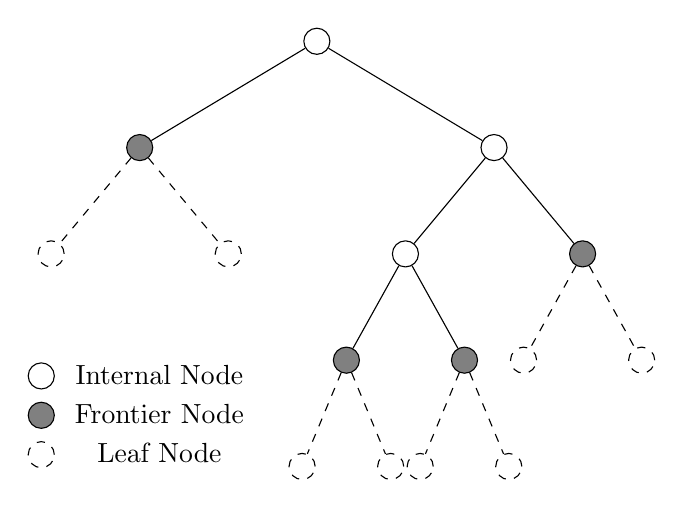
\begin{tikzpicture}[scale=.9,level/.style={sibling distance=50mm/#1}]
\node [circle,draw] (z) {}
  child {node [circle,draw,fill=gray] (a) {}
    child[dashed] {node [circle,draw,dashed] (b) {}}
    child[dashed] {node [circle,draw,dashed] (g) {}}
  }
  child {node [circle,draw] (j) {}
    child {node [circle,draw] (k) {}
      child {node [circle,draw,fill=gray] (o) {}
        child[dashed] {node [circle,draw,dashed] (x) {}}
        child[dashed] {node [circle,draw,dashed] (y) {}}
      }
      child {node [circle,draw,fill=gray] (p) {}
        child[dashed] {node [circle,draw,dashed] (x) {}}
        child[dashed] {node [circle,draw,dashed] (y) {}}
      }
    }
  child {node [circle,draw,fill=gray] (l) {}
    child[dashed] {node [circle,draw,dashed] (c) {}}
    child[dashed] {node [circle,draw,dashed] (d) {}}
  }
};

\node [shift={(-3.5,-4.25)},circle,draw,label={[xshift=1.5cm, yshift=-0.4cm] Internal Node}] (leg1) {};
\node [shift={(-3.5,-4.75)},circle,draw,fill=gray,label={[xshift=1.5cm, yshift=-0.4cm] Frontier Node}] (leg1) {};
\node [shift={(-3.5,-5.25)},circle,draw,dashed,label={[xshift=1.5cm, yshift=-0.4cm] Leaf Node}] (leg1) {};
\end{tikzpicture}
}
\caption{Hierarchy node classification}
\label{fig:tree}
\end{figure}

Our hierarchical clustering algorithm is presented in \Cref{alg:hiernmf2} and follows that of Kuang and Park \cite{KP13}.
Each node includes a field $\M{A}$, which is a subset of columns (samples) of the original data, a feature vector $\V{w}$, which is its corresponding column of the $\M{W}$ matrix from its parent's Rank-2 NMF, a score, and pointers to its left and right children.
A priority queue $\cal Q$ tracks the frontier nodes so that the node with the highest score is split at each step of the algorithm.
We use a target number of leaf clusters $k$ as the termination condition.
When a node is selected from the priority queue, it is removed from the set of frontier nodes and its children are added.

\begin{algorithm}
\caption{Hierarchical Clustering \cite{KP13}}
\label{alg:hiernmf2}
\begin{algorithmic}[1]
	\Require{$\M{A}$ is $m\times n$, $k$ is target number of leaf clusters}
	\Function{${\cal T} =$ Hier-R2-NMF}{$\M{A}$}
		\State ${\cal R} = \text{node}(\M{A})$ \hfill \Comment{create root node}
		\State \textsc{Split}$({\cal R})$
		\State inject$({\cal Q},{\cal R}.\text{left})$ \hfill \Comment{create priority queue}
		\State inject$({\cal Q},{\cal R}.\text{right})$ \hfill \Comment{of frontier nodes}
		\While{size$({\cal Q}) < k$}
			\State ${\cal N} = \text{eject}({\cal Q})$ \hfill \Comment{frontier node with max score}
			\State \textsc{Split}$({\cal N}.\text{left})$ \hfill \Comment{split left child}
			\State inject$({\cal Q},{\cal N}.\text{left})$ \hfill \Comment{and add to $\cal Q$}
			\State \textsc{Split}$({\cal N}.\text{right})$ \hfill \Comment{split right child}
			\State inject$({\cal Q},{\cal N}.\text{right})$ \hfill \Comment{and add to $\cal Q$}
		\EndWhile
	\EndFunction
	\Ensure{$\cal{T}$ is binary tree rooted at $\cal R$ with $k$ frontier nodes, each node has subset of cols of $\M{A}$ and feature vector $\V{w}$}
\end{algorithmic}
\end{algorithm}

The splitting procedure is specified in \Cref{alg:split}.
After the Rank-2 NMF is performed, the $\M{H}$ factor is used to determine part membership, and the columns of the $\M{W}$ factor are assigned to the child nodes.
The score of the node is computed as the reduction in overall NMF error if the node is split, which can be computed from the principal singular values of the subsets of columns of the node and its children.
The principal singular values of the children are computed via the power method (the principal singular value of the node was computed when its parent's score was computed).

\begin{algorithm}
\caption{Node Splitting via Rank-Two NMF}
\label{alg:split}
\begin{algorithmic}[1]
	\Require{$\cal N$ has a subset of columns given by field $\M{A}$}
	\Function{Split}{$\cal N$}
		\State $[\M{W},\M{H}] = \textsc{Rank2-NMF}({\cal N}.\M{A})$ \hfill \Comment{split $\cal N$}
		\State partition ${\cal N}.\M{A}$ into $\M{A}_1$ and $\M{A}_2$ using $\M{H}$
		\State ${\cal N}.\text{left} = \text{node}(\M{A}_1,\V{W}_1)$ \hfill \Comment{create left child}
		\State ${\cal N}.\text{right} = \text{node}(\M{A}_2,\V{W}_2)$ \hfill \Comment{create right child}
		\State ${\cal N}.\text{score} = \sigma_1^2(\M{A}_1) + \sigma_1^2(\M{A}_2) - \sigma_1^2({\cal N}.\M{A})$
	\EndFunction
	\Ensure{$\cal{N}$ has two children and a score}
\end{algorithmic}
\end{algorithm}

\subsection{Parallelization}

In this section, we consider the options for parallelizing Hierarchical Rank-2 NMF Clustering (\Cref{alg:hiernmf2}) and provide an analysis for the approach we take.
The running time of an algorithm is data dependent because not only does each Rank-2 NMF computation require a variable number of iterations, but also the shape of the tree can vary from a balanced binary tree with $O(\log k)$ levels to a tall, flat tree with $O(k)$ levels.
For the sake of analysis, we will assume a fixed number of NMF iterations for every node of the tree and we will analyze the cost of complete levels.

The first possibility for parallelization is across the nodes of the tree, as each Rank-2 NMF split is independent.
We choose not to parallelize across nodes in the tree for two reasons.
The first reason is that while the NMF computations are independent, choosing which nodes to split may depend on global information.
In particular, when the global target is to determine $k$ leaf clusters, the nodes must be split in order of their scores, which leads to a serialization of the node splits.
This serialization might be relaxed using speculative execution, but it risks performing unnecessary computation.
If the global target is to split all nodes with sufficiently high scores, then this serialization is also avoided and node splits become truly independent.
We choose not to parallelize in this way to remain agnostic to the global stopping criterion.

The second reason is that parallelizing across nodes requires redistribution of the input data.
Given a node split by $\hat p$ processors, in order to assign disjoint sets of processors to each child node, each of the $\hat p$ processors would have to redistribute their local data, sending data for samples not in their child's set and receiving data for those in their child's set.
The communication would be data dependent, but on average, each processor would communicate half of its data in the redistribution set, which could have an all-to-all communication pattern among the $\hat p$ processors.
For a node with $\hat n$ columns, the communication cost would be at least $O(m\hat n/ \hat p)$ words, which is much larger than the communication cost per iteration of Parallel Rank-2 NMF, as we will see in \Cref{sec:analysis}.

By choosing not to parallelize across nodes in the tree, we employ all $p$ processors on each node, and split nodes in sequence.
The primary computations used to split a node are the Rank-2 NMF and the score computation, which is based on an approximation of the largest singular value.
We use an alternating-updating algorithm for Rank-2 NMF as described in \Cref{sec:prelim}, and we parallelize it following the methodology proposed in \cite{EH+19-TR} and presented in \Cref{alg:parrank2nmf}.

The communication cost of the algorithm depends on the parallel distribution of the input matrix data $\M{A}$.
In order to avoid redistribution of the matrix data, we choose a 1D row distribution so that each processor owns a subset of the rows of $\M{A}$.
Because the clustering partition splits the columns of $\M{A}$, each processor can partition its local data into left and right children to perform the split without any interprocessor communication.
If we use a 2D distribution for a given node, then because the partition is data dependent, a data redistribution is required in order to obtain a load balanced distribution of both children.
\Cref{fig:split} presents a visualization of the node-splitting process using a 1D processor distribution.
In the following subsections, we describe the parallel algorithms for Rank-2 NMF and approximating the principal singular value given this 1D data distribution and analyze their complexity in the context of the hierarchical clustering algorithm.

\begin{figure}
%!TEX root = ../paper.tex

\newcommand{\lightred}{red!75}
\newcommand{\lightblue}{blue!75}
\newcommand{\offset}{.1}

\begin{tikzpicture}

% draw A
\fill[\lightred] (0,0) rectangle ++(0.5,4);
\fill[\lightblue] (0.5,0) rectangle ++(1.25,4);
\fill[\lightred] (1.75,0) rectangle ++(1.25,4);
\fill[\lightblue] (3,0) rectangle ++(1,4);
\draw[thick,dashed,xscale=4,yscale=4/3] (0,0) grid ++(1,3);
\draw[very thick] (0,0) rectangle (4,4);
\node at (2,-3*\offset) {$\M{A}$};

% draw W
\draw[fill=\lightred,shift={(-.5,0)}] (0,0) rectangle ++ (.15,4);
\draw[fill=\lightblue,shift={(-.5,0)}] (.15,0) rectangle ++ (.15,4);
\draw[thick,shift={(-.5,0)},xscale=.15,yscale=4] (0,0) grid ++(2,1);
\node at (-.5+.15,-3*\offset) {$\M{W}$};

% draw H
\draw[thick,shift={(0,4.1)},xscale=4,yscale=.15] (0,0) grid ++(1,2);
\node at (4+4*\offset,4.3) {$\M{H}^\Tra$};
\draw[fill=\lightred,shift={(0,4.1)}] (0,.15) rectangle ++(.5,.15);
\draw[fill=\lightblue,shift={(0,4.1)}] (.5,0) rectangle ++(1.25,.15);
\draw[fill=\lightred,shift={(0,4.1)}] (1.75,.15) rectangle ++(1.25,.15);
\draw[fill=\lightblue,shift={(0,4.1)}] (3,0) rectangle ++(1,.15);

\begin{scope}[shift={(-1,-6)}]
	% draw A_1 and w_1
	\draw[very thick,fill=\lightred] (0,0) rectangle ++(2.25,4);
	\draw[thick,dashed,xscale=2.25,yscale=4/3] (0,0) grid ++(1,3);
	\node at (1.125,-3*\offset) {$\M{A}_1$};
	\draw[thick,fill=\lightred] (-.5,0) rectangle ++(.15,4);
	\node at (-.5+.15,-3*\offset) {$\V{W}_1$};
	
	% draw A_2 and w_2
	\draw[very thick,fill=\lightblue] (5,0) rectangle ++(1.75,4);
	\draw[thick,dashed,shift={(5,0)},xscale=1.75,yscale=4/3] (0,0) grid ++(1,3);
	\node at (5.875,-3*\offset) {$\M{A}_2$};
	\draw[thick,,fill=\lightblue,shift={(5,0)}] (-.5,0) rectangle ++(.15,4);
	\node at (5-.5+.15,-3*\offset) {$\V{W}_2$};
\end{scope}

% draw arrows to A_1 and w_1
% TODO: make these arrows prettier
\draw[thick] (0.25,-\offset) parabola (.125,-0.5);
\draw[thick] (2.25,-\offset) parabola (.125,-0.5);
\draw[thick,->] (.125,-0.5) parabola (.125,-2+\offset);
\draw[thick,->] (-.5+.075,-\offset) parabola (-1.5+.075,-2+\offset);

% draw arrows to A_2
% TODO: make these arrows prettier
\draw[thick] (1,-\offset) parabola (4.375,-0.5);
\draw[thick] (3.5,-\offset) parabola (4.375,-0.5);
\draw[thick,->] (4.375,-0.5) parabola (4.875,-2+\offset);
\draw[thick,->] (-.5+.225,-\offset) parabola (3.5+.075,-2+\offset);

\end{tikzpicture}

\caption{Parallel splitting using Rank-2 NMF and 1D processor distribution.  A Rank-2 NMF computes factor matrices $\M{W}$ and $\M{H}$ to approximate $\M{A}$, the values of $\M{H}$ are used to determine child membership of each column (either red or blue), and the corresponding column of the $\M{W}$ matrix represents the part's feature weighting.  The 1D distribution is depicted for 3 processors to show that the splitting requires no interprocessor redistribution as the children are evenly distributed identically to the parent.}
\label{fig:split}
\end{figure}

\subsubsection{Algorithms}

\paragraph{\emph{Parallel Rank-2 NMF}}

\Cref{alg:parrank2nmf} presents the parallelization of an alternating-updating scheme for NMF that uses the exact rank-2 solve algorithm presented in \Cref{alg:r2nnls} to update each factor matrix.
The algorithm computes the inputs to the rank-2 solves in parallel and then exploits the parallelism across rows of the factor matrix so that each processor solves for a subset of rows simultaneously.
The distribution of all matrices is 1D row distribution, so that each processor owns a subset of the rows of $\M{A}$, $\M{W}$, and $\M{H}$.
We use the notation $\M[\hat]{A}$ to refer to the $(m/p) \times n$ local data matrix and $\M[\hat]{W}$ and $\M[\hat]{H}$ to refer to the $(m/p) \times 2$ and $(n/p)\times 2$ local factor matrices.
With this distribution, the computation of $\M{W}^\Tra\M{W}$ and $\M{H}^\Tra\M{H}$ each is done via local multiplication followed by a single all-reduce collective.
All processors own the data they need to compute their contribution to $\M{A}^\Tra \M{W}$; in order to distribute the result to compute the rows $\M{H}$ independently, a reduce-scatter collective is used to sum and simultaneously distribute across processors.
To obtain the data needed to compute $\M[\hat]{W}$, each processor must access all of $\M{H}$, which is performed via an all-gather collective.
The iteration progresses until a convergence criterion is satisfied.
For performance benchmarking we use a fixed number of iterations, and in practice we use relative change in objective function value (residual norm).

\begin{algorithm}
\caption{Parallel Rank-2 NMF}
\label{alg:parrank2nmf}
\begin{algorithmic}[1]
	\Require{$\M{A}$ is $m\times n$ and row-distributed across processors so that $\M[\hat]{A}$ is local $(m/p)\times n$ submatrix}
	\Function{$[\M{W},\M{H}] =$ Parallel-Rank2-NMF}{$\M{A}$}
		\State Initialize local $\M[\hat]{W}$ randomly
		\While{not converged}
			\State \Comment{Compute $\M{H}$}
			\State $\M[\hat]{G}_W = \M[\hat]{W}^\Tra \M[\hat]{W}$
			\State $\M{G}_W = \textsc{All-Reduce}(\M[\hat]{G})$
			\State $\M[\hat]{B} = \M[\hat]{A}^\Tra \M[\hat]{W}$ %\hfill \Comment{local matrix multiplication}
			\State $\M[\hat]{C} = \textsc{Reduce-Scatter}(\M[\hat]{B})$
			\State $\M[\hat]{H} = \textsc{Rank2-NLS-Solve}(\M[\hat]{C},\M{G}_W)$
			\State \Comment{Compute $\M{W}$}
			\State $\M[\hat]{G}_H = \M[\hat]{H}^\Tra \M[\hat]{H}$
			\State $\M{G}_H = \textsc{All-Reduce}(\M[\hat]{G}_H)$
			\State $\M{H} = \textsc{All-Gather}(\M[\hat]{H})$
			\State $\M[\hat]{D} = \M[\hat]{A} \M{H}$ %\hfill \Comment{local matrix multiplication}
			\State $\M[\hat]{W} = \textsc{Rank2-NLS-Solve}(\M[\hat]{D},\M{G}_H)$
		\EndWhile
	\EndFunction
	\Ensure{$\M{A} \approx \M{W}\M{H}^\Tra$ with $\M{W}$, $\M{H}$ row-distributed}
\end{algorithmic}
\end{algorithm}

\paragraph{\emph{Parallel Power Method}}

In order to compute the score for a frontier node, we use the difference between the principal singular value of the matrix columns of the node and the sum of those of its children.
Thus, we must determine the principal singular value of every node in the tree once, including leaf nodes.
We use the power method to approximate it, repeatedly applying $\M{A}\M{A}^\Tra$ to a vector until it converges to the leading right singular vector.
We present the power method in \Cref{alg:parpowmeth}.
Note that we do not normalize the approximate left singular vector so that the computed value approximates the square of the largest singular value.

Given the 1D distribution, only one communication collective is required for the pair of matrix-vector multiplications.
That is, the approximate right singular vector $\V{v}$ is redundantly owned on each processor, and the approximate left singular vector $\V{u}$ is distributed across processors.
Each processor can compute its local $\V[\hat]{u}$ from $\V{v}$ without communication and use the result for its contribution to $\V{v}=\M{A}^\Tra \V{u}$.
An all-reduce collective is used to obtain a copy of $\V{v}$ on every processor for the next iteration, and the norm is redundantly computed without further communication.
Again, we use a fixed number of iterations for benchmarking, but the more practical stopping criterion is based on the relative change in $\sigma$.

\begin{algorithm}
\caption{Parallel Power Method}
\label{alg:parpowmeth}
\begin{algorithmic}[1]
	\Require{$\M{A}$ is $m\times n$ and row-distributed across processors so that $\M[\hat]{A}$ is local $(m/p)\times n$ submatrix}
	\Function{$\sigma =$ Parallel-Power-Method}{$\M{A}$}
		\State Initialize $\V{v}$ randomly and redundantly
		\While{not converged}
			\State $\V[\hat]{u} = \M[\hat]{A} \V{v}$
			\State $\V[\hat]{z} = \M[\hat]{A}^\Tra \V[\hat]{u}$
			\State $\V{v} = \textsc{All-Reduce}(\V[\hat]{z})$
			\State $\sigma = \|\V{v}\|$
			\State $\V{v} = \V{v}/\sigma$
		\EndWhile
	\EndFunction
	\Ensure{$\sigma \approx \sigma_1^2(\M{A})$ is  redundantly owned by all procs}
\end{algorithmic}
\end{algorithm}


\subsubsection{Analysis}
\label{sec:analysis}

\paragraph{\emph{Parallel Rank-2 NMF}}

Each iteration of \Cref{alg:parrank2nmf} incurs the same cost, so we analyze per-iteration computation and communication costs.
We first consider the cost of the Rank-2 NNLS solves, which are local computations.
In the notation of \Cref{alg:r2nnls}, matrix $\M{G}$ is $2\times 2$, so solving the unconstrained system (via Cholesky decomposition) and then choosing between single-positive-variables solutions if necessary requires constant time per row of $\M{C}$.
Thus, the cost of \Cref{alg:r2nnls} is proportional to the number of rows of the first input matrix.
In the context of \Cref{alg:parrank2nmf}, the per-iteration computational cost of rank-2 solves is then $O((m+n)/p)$.
The other local computations are the matrix multiplications $\M[\hat]{W}^\Tra \M[\hat]{W}$ and $\M[\hat]{H}^\Tra \M[\hat]{H}$, which also amount to $O((m+n)/p)$ flops, and $\M[\hat]{A}^\Tra \M[\hat]{W}$ and $\M[\hat]{A} \M{H}$, which require $O(mn/p)$ flops because they involve the data matrix.
Thus, the computation cost is $\gamma \cdot O((mn+m+n)/p)$ and typically dominated by the multiplications involving $\M{A}$.
We track the lower order terms corresponding to NNLS solves because their hidden constants are larger than that of the dominating term.

There are four communication collectives each iteration, and each involves all $p$ processors.
The two all-reduce collectives to compute the Gram matrices of the factor matrices involve $2\times 2$ matrices and incur a communication cost of $(\beta + \alpha) \cdot O(\log p)$.
The reduce-scatter and all-gather collectives involve $n\times 2$ matrices (the size of $\M{H}$) and require $\beta \cdot O(n) + \alpha \cdot O(\log p)$ in communication cost (we ignore the computation cost of the reduce-scatter because it is typically dominated by the bandwidth cost).
If the algorithm performs $\imath$ iterations, the overall cost of \Cref{alg:parrank2nmf} is
\begin{equation}
\label{eq:r2nmfcost}
\gamma \cdot O\left( \frac{\imath (mn+m+n)}{p} \right) + \beta \cdot O(\imath n) + \alpha \cdot O(\imath \log p).
\end{equation}

\paragraph{\emph{Parallel Power Method}}

Similar to the previous analysis, we consider a single iteration of the power method.
The local computation is dominated by two matrix-vector products involving the local data matrix of size $O(mn/p)$ words, incurring $O(mn/p)$ flops.
The single communication collective is an all-reduce of the approximate right singular vector, which is of size $n$, incurring $\beta \cdot O(n) + \alpha \cdot O(\log p)$ communication.
We ignore the $O(n)$ computation cost of normalizing the vector, as it will typically be dominated by the communication cost of the all-reduce.
Over $\jmath$ iterations, \Cref{alg:parpowmeth} has an overall cost of
\begin{equation}
\label{eq:powmethcost}
\gamma \cdot O\left( \frac{\jmath mn}{p} \right) + \beta \cdot O(\jmath n) + \alpha \cdot O(\jmath \log p).
\end{equation}
Note the per-iteration cost of the power method differs by only a constant from the per-iteration cost of Rank-2 NMF.
Because the power method involves single vectors rather than factor matrices with two columns, its constants are smaller than half the size of their counterparts.

\paragraph{\emph{Hierarchical Clustering}}

To analyze the overall cost of the hierarchical clustering algorithm, we sum the costs over all nodes in the tree.
Because the shape of the tree is data dependent and affects the overall costs, for the sake of analysis we will analyze only complete levels.
The number of rows in any node is $m$, the same as the root node, as each splitting corresponds to a partition of the columns.
Furthermore, because each split is a partition, every column of $\M{A}$ is represented exactly once in every complete level of the tree.
If we assume that all nodes perform the same number of NMF iterations ($\imath$) and power method iterations $(\jmath)$, then the dominating costs of a node with $\overline{n}$ columns is
\begin{equation*}
\label{eq:nodecost}
\begin{split}
\gamma \cdot O\left( \frac{(\imath+\jmath) m\overline{n} + \imath (m+\overline{n}) }{p} \right) + \beta \cdot O((\imath+\jmath) \overline{n}) \\ + \alpha \cdot O((\imath+\jmath) \log p).
\end{split}
\end{equation*}
Because the sum of the number of columns across any level of the tree is $n$, the cost of the $\ell$th level of the tree is
\begin{equation}
\label{eq:levelcost}
\begin{split}
\gamma \cdot O\left( \frac{(\imath+\jmath) mn + \imath m 2^\ell}{p} \right) + \beta \cdot O((\imath+\jmath) n) \\ + \alpha \cdot O((\imath+\jmath) 2^\ell \log p).
\end{split}
\end{equation}
Note that the only cost that depends on the level index $\ell$ is the latency cost.
Summing over levels and assuming the tree is nearly balanced and has height $O(\log k)$ where $k$ is the number of frontier nodes, we obtain an overall cost of \Cref{alg:hiernmf2} of
\begin{equation}
\label{eq:treecost}
\begin{split}
\gamma \cdot O\left( \frac{(\imath+\jmath) mn}{p}  \log k + \frac{\imath mk}{p} \right) + \beta \cdot O((\imath+\jmath) n \log k) \\ + \alpha \cdot O((\imath+\jmath) k \log p).
\end{split}
\end{equation}

We see that the leading order computational cost is logarithmic in $k$ and perfectly load balanced.
If the overall running time is dominated by the computation (and in particular the matrix multiplications involving $\M{A}$), we expect near-perfect strong scaling.
The bandwidth cost is also logarithmic in $k$ but does not scale with the number of processors.
The latency cost grows most quickly with the target number of clusters $k$ but is also independent of the matrix dimensions $m$ and $n$.

\section{Experimental Results}

\subsection{Experimental Platform}
All the experiments in this section were conducted on Summit. Summit is a supercomputer created by IBM for the Oak Ridge National Laboratory. 
There are approximately 4,600 nodes on Summit. Each node contains two IBM POWER9 processors on separate sockets with dual NVLINK bricks to facilitate a transfer rate of 
25 GB/s between the processors. Each node contains 512 GB of DDR4 memory for use by both processors. Each POWER9 processor utilizes 22 IBM SIMD Multi-Cores (SMCs), 
although one of these SMCs on each processor is dedicated to memory transfer and is therefore not available for computation. 
For node scaling experiments, all 42 available SMCs were utilized in each node so that every node computed with 42 separate MPI processes.
Additionally, every node also supports six NVIDIA Volta V100 accelerators but these were unused by our algorithm. 

H2NMF uses the Armadillo library (version 9.900.1) for all matrix operations. 
In Armadillo, sparse matrices are stored in Compressed Sparse Column (CSC) format and dense matrices are stored in column-major ordering.
On Summit, we linked this version of Armadillo with OpenBLAS (version 0.3.9) and IBM's Spectrum MPI (version 10.3.1.2-20200121).


\GB{specify that $\imath=\jmath=100$ in all experiments, also what do we set $k$ to be?  fixed number for each dataset?  any other experimental parameters we should specify? could also specify these at the beginning of \Cref{sec:perf}}


\subsection{Datasets}

\GB{need shortcut names for datasets: synthetic, DC, and something better than IMAGE}

\begin{itemize}
	\item \textit{Document Clustering}:
	These datasets are represented by sparse matrices in term frequency-inverdse document frequency (TFIDF) format.
	The rows of these matrices represent words and the columns represent individual documents. Each value in the matrix is a TFIDF statistic for
	a specific word in a document. 

	For H2NMF, we used two popular document clustering datasets: Reuters Newswire Topic Classification (Reuters-21578) and \dots
	\LM{I can't find the official name for PubMed or a link to it}

	The Reuters matrix is $12411\times 7984$ and is a preprocessed version of Reuters-21578 used in the SmallK implementation of H2NMF.
	The preprocessed version is the 20 largest prelabeled classes of documents with only single class labels. 
	\LM{Prof Park, is this explanation of Reuters correct?}
	As Reuters is small, it is mainly used as a comparison tool between the ours and the SmallK implmentation.

	The PubMed matrix is $141043\times 8200000$. It is not preprocessed and represents the full size dataset in TFIDF format. This version is
	better suited for scaling as is it is much larger than Reuters and is a good representation of large text classification datasets.

	\item \textit{Hyperspectral Imaging}:
	The images chosen for this dataset follow a similar pattern to Document Clustering. We chose two datasets: the Hyperspectral digital imagery
	collection experiment (HYDICE) image of the Washington DC Mall and the Airborne Visible/Infrared Image Spectrometer (AVIRIS) image 
	of the DC area. 

	The images are formatted into 3-way tensors representing individual images in each spectral band captured. For H2NMF, these tensors 
	are flattened so that the rows represent spectral bands (191 for HYDICE and 224 for AVIRIS) and the columns represent pixels.

	The HYDICE image is flattened from $1280\times 307\times 191$ to $191\times 392960$ and the AVIRIS image is likewise
	flattened from $8940\times 747\times 224$ to $224\times 6678180$. Unlike with document clustering, hyperspectral image sizes grow in pixels
	and not spectral bands. So, for both images, large scaling is impossible given our current data distribtion.
	\LM{I think this is awkward and I'm not sure if we need to include it}
	

	\LM{DC: https://engineering.purdue.edu/~biehl/MultiSpec/hyperspectral.html}

	\LM{AVIRIS: https://aviris.jpl.nasa.gov/dataportal/}

	

	\item synthetic (dense and sparse)
	\item HSI: DC and Aviris
	\item Doc-clustering: Reuters and PubMed
\end{itemize}

\subsection{Performance}
\label{sec:perf}

\subsubsection{Rank-2 NMF Strong Scaling}

We perform strong scaling experiments for a single Rank-2 NMF (\Cref{alg:parrank2nmf}) on the synthetic and IMAGE datasets.
The theory (\Cref{eq:r2nmfcost}) suggests that perfect strong scaling is possible as long as the execution time is dominated by local computation.
Both the matrix multiplications and NNLS solves scale linearly with $1/p$ (we expect MatMul to dominate), but the bandwidth cost is independent of $p$ and the latency cost increases slightly with $p$.

\Cref{fig:synrank2speedup,fig:rwrank2speedup} show performance relative to the smallest number of nodes required to store data and factor matrices.
The synthetic data is chosen to fit on a single node, while the IMAGE data requires 10 nodes to store the input matrix as well as temporary and output matrices.
For these data sets, we observe nearly perfect strong scaling, with 47$\times$ speedup on 50 nodes (over 1 node) for synthetic data and 7.1$\times$ speedup on 80 nodes (over 10 nodes) for IMAGE data.

\begin{figure}
\begin{center}
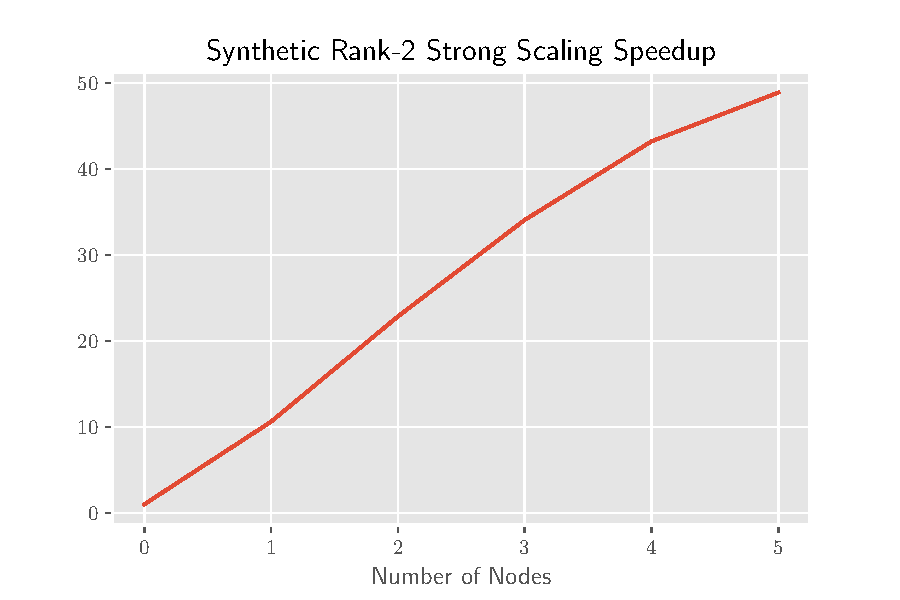
\includegraphics[height=2in, width=\columnwidth]{plots/synthetic_rank2_speedup.pdf}
\caption{Strong Scaling Speedup for Rank-2 NMF on synthetic data}
\label{fig:synrank2speedup}
\end{center}
\end{figure}

\begin{figure}
\begin{center}
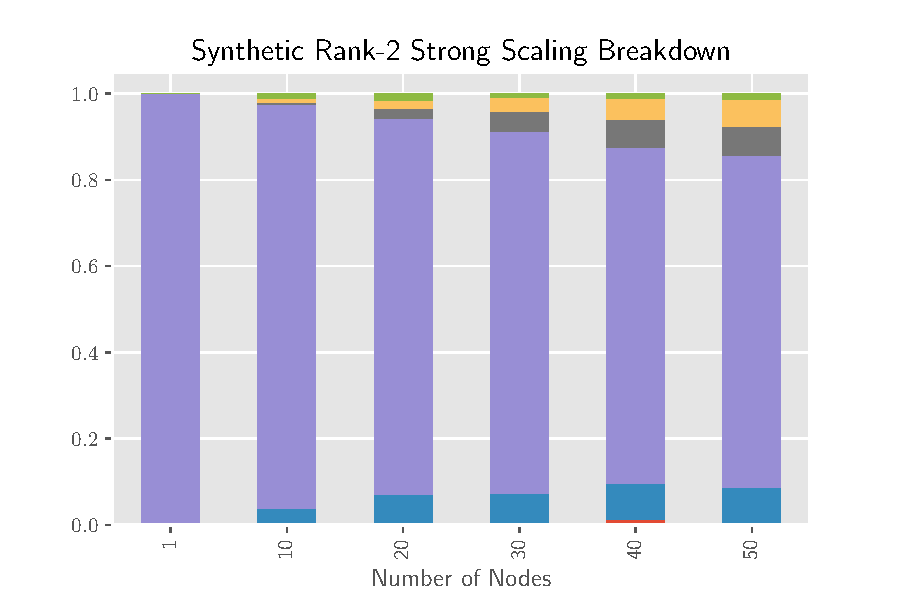
\includegraphics[height=2in, width=\columnwidth]{plots/synthetic_rank2_strongscaling.pdf}
\caption{Relative Time Breakdown for Rank-2 NMF on synthetic data}
\label{fig:synrank2strongscaling}
\end{center}
\end{figure}

The relative time breakdowns are presented in \Cref{fig:synrank2strongscaling,fig:rwrank2strongscaling} and explain the strong scaling performance.
Each experiment is normalized to 100\% time, so comparisons cannot be readily made across numbers of compute nodes. 
For both data sets, we see that the time is dominated by MatMul, which is the primary reason for the scalability.
The dominant matrix multiplications are between a large matrix and a matrix with 2 columns, so it is locally memory bandwidth bound, with performance proportional to the size of the large matrix.
In each plot, we also see the relative time of all-gather and reduce-scatter increasing, which is because the local computation is decreasing while the communication cost is slightly increasing with $p$.
This pattern will continue as $p$ increases, which will eventually limit scalability, but for these data sets the MatMul takes around 80\% of the time at over 2000 cores.

\begin{figure}
\begin{center}
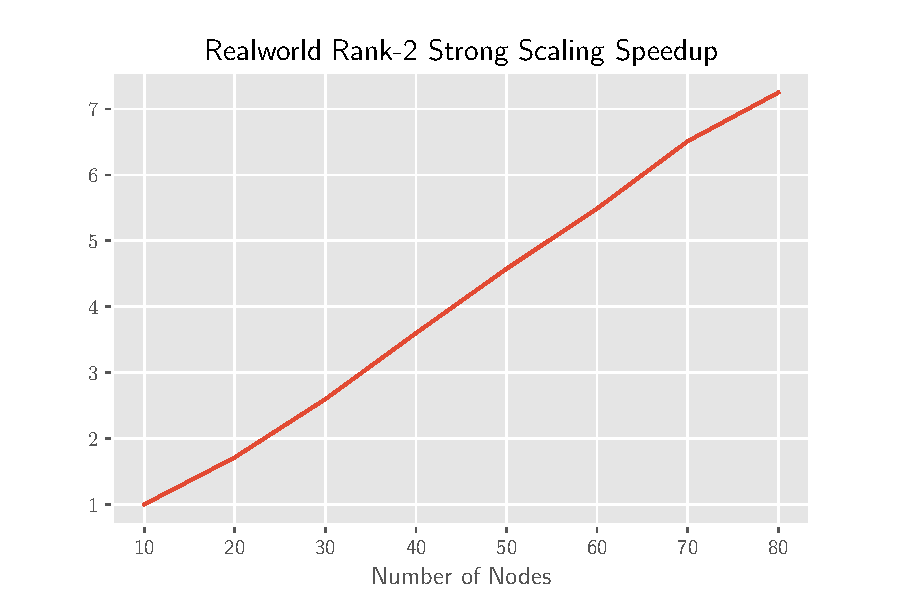
\includegraphics[height=2in, width=\columnwidth]{plots/realworld_rank2_speedup.pdf}
\caption{Strong Scaling Speedup for Rank-2 NMF on IMAGE data}
\label{fig:rwrank2speedup}
\end{center}
\end{figure}

\begin{figure}
\begin{center}
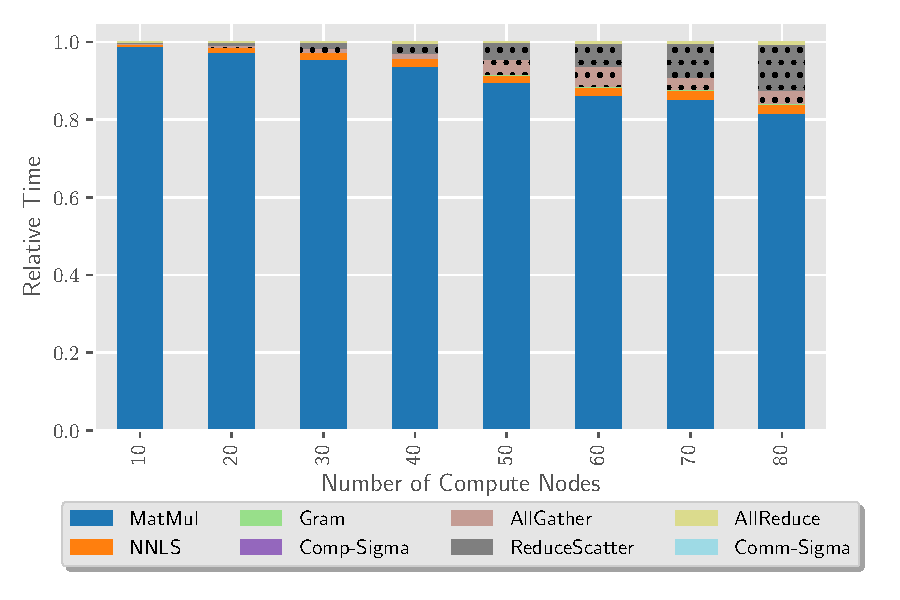
\includegraphics[height=2in, width=\columnwidth]{plots/realworld_rank2_strongscaling.pdf}
\caption{Relative Time Breakdown for Rank-2 NMF on IMAGE data}
\label{fig:rwrank2strongscaling}
\end{center}
\end{figure}



\subsubsection{Hierarchical Clustering Strong Scaling}

\GB{Do these breakdowns include the score function?  actually this may explain why all-reduce costs more, it also has $O(n)$ data for score...}

\GB{4 plots: 2 data sets with speedup/breakdown, note that we include time for complete levels, ignoring nodes in incomplete levels for easier interpretation}

\begin{itemize}
	\item theory (\Cref{eq:treecost}) says...
	\item Fig 7 shows limit of strong scaling for synthetic data (time increases at 50 nodes compared to 40), Fig 8 gives breakdown and explains
	\begin{itemize}
		\item drastic performance dropoff may be artifact of all-gather, which should take about the same time as reduce-scatter, but speedup from 30 to 40 nodes is also slight
		\item by 50 nodes, about 50\% of time in communication; still mostly dominated by bandwidth cost because ag and rs dominate ar
		\item note the difference between the scaling of single rank-2 and entire tree: poor scaling must be due to lower levels, which we explore in the next section
	\end{itemize}
	\item Fig 9 shows reasonable scaling for entire tree -- speedup drops from 7x to 6x over 80 nodes; Fig 10 shows that MM is still 70\% of run time on 80 nodes, which allows for near-linear scaling
\end{itemize}

\begin{figure}
\begin{center}
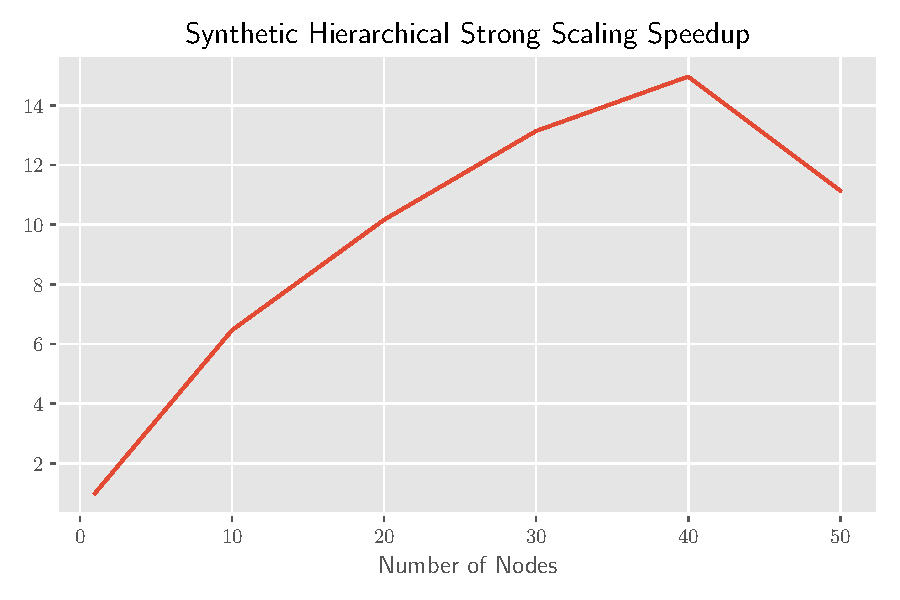
\includegraphics[height=2in, width=\columnwidth]{plots/synthetic_hierarchical_speedup.pdf}
\caption{Strong Scaling Speedup for Hierarchical Clustering. The total time taken for complete Hierarchical Clustering \cref{alg:hiernmf2}}
\label{fig:synhierspeedup}
\end{center}
\end{figure}

\begin{figure}
\begin{center}
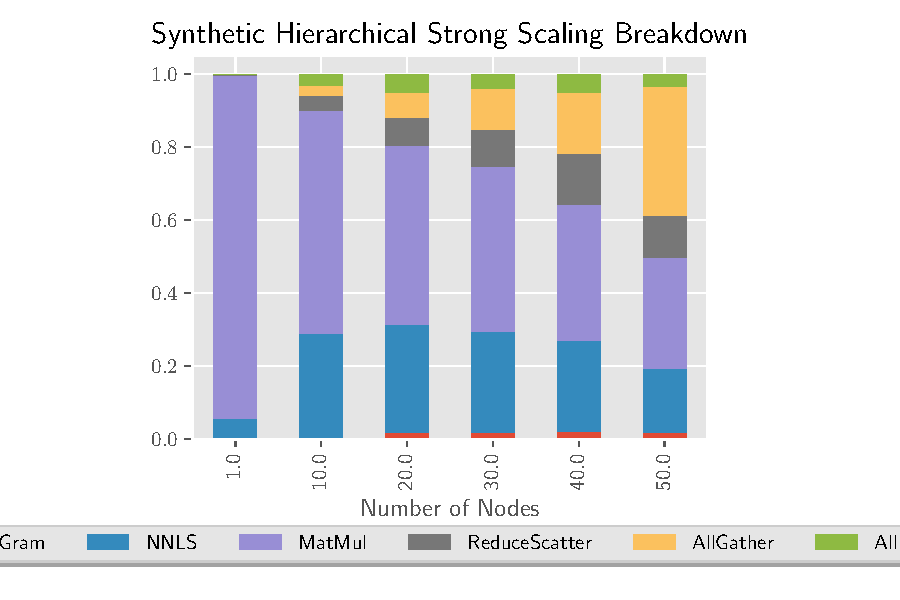
\includegraphics[height=2in, width=\columnwidth]{plots/synthetic_hier_strongscaling.pdf}
\caption{Relative Time Breakdown for Hierarchical Clustering. The plot uses the total time taken for complete Hierarchical Clustering \cref{alg:hiernmf2}}
\label{fig:synhierstrongscaling}
\end{center}
\end{figure}

\begin{figure}
\begin{center}
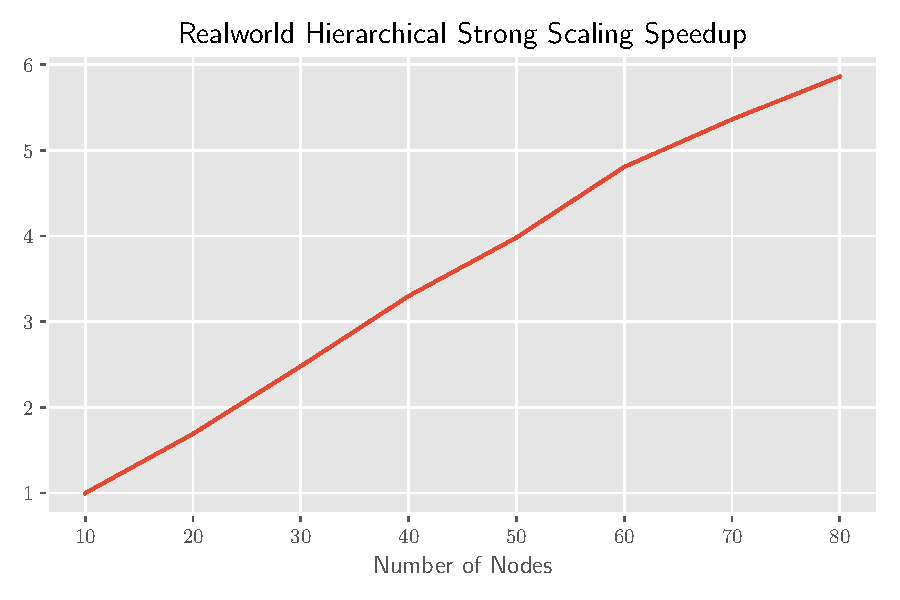
\includegraphics[height=2in, width=\columnwidth]{plots/realworld_hierarchical_speedup.pdf}
\caption{Strong Scaling Speedup for Hierarchical Clustering on Realworld Data. The total time taken for complete Hierarchical Clustering \cref{alg:hiernmf2}}
\label{fig:rwhierspeedup}
\end{center}
\end{figure}

\begin{figure}
\begin{center}
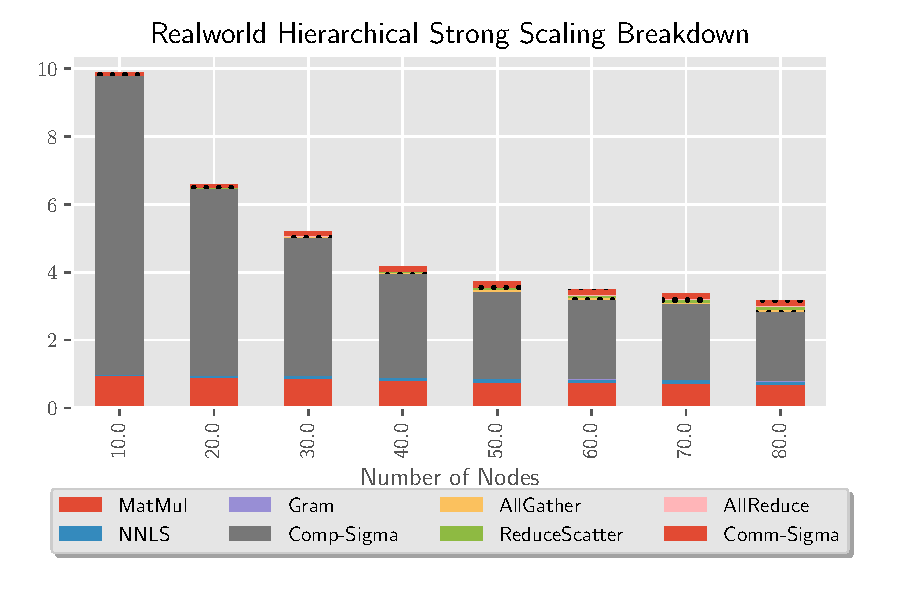
\includegraphics[height=2in, width=\columnwidth]{plots/realworld_hier_strongscaling.pdf}
\caption{Relative Time Breakdown for Hierarchical Clustering on Realworld. The plot uses the total time taken for complete Hierarchical Clustering \cref{alg:hiernmf2}}
\label{fig:rwhierstrongscaling}
\end{center}
\end{figure}

\subsubsection{Level Scaling}

\GB{3 plots: for synthetic level breakdown for 1 node and for 40 nodes; for realworld just for 80 nodes}

\begin{itemize}
	\item theory says per-level cost is \Cref{eq:levelcost}
\end{itemize}

\begin{figure}
\begin{center}
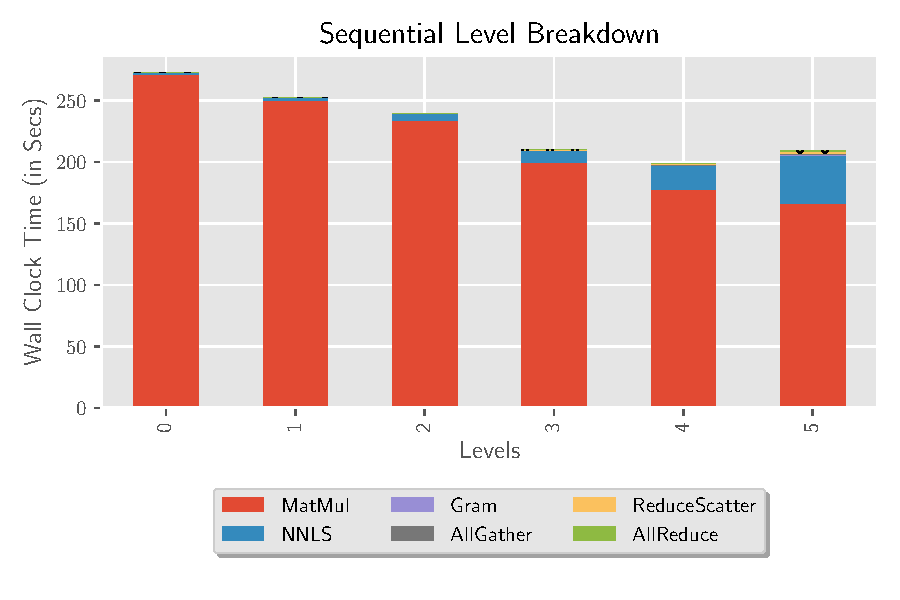
\includegraphics[height=2in, width=\columnwidth]{plots/synthetic_sequential_level_breakdown.pdf}
\caption{Sequential Breakdown plot for levels 0 to 5. y-axis is absolute wall clock time in seconds}
\label{fig:seqlevelbreakdown}
\end{center}
\end{figure}

\begin{figure}
\begin{center}
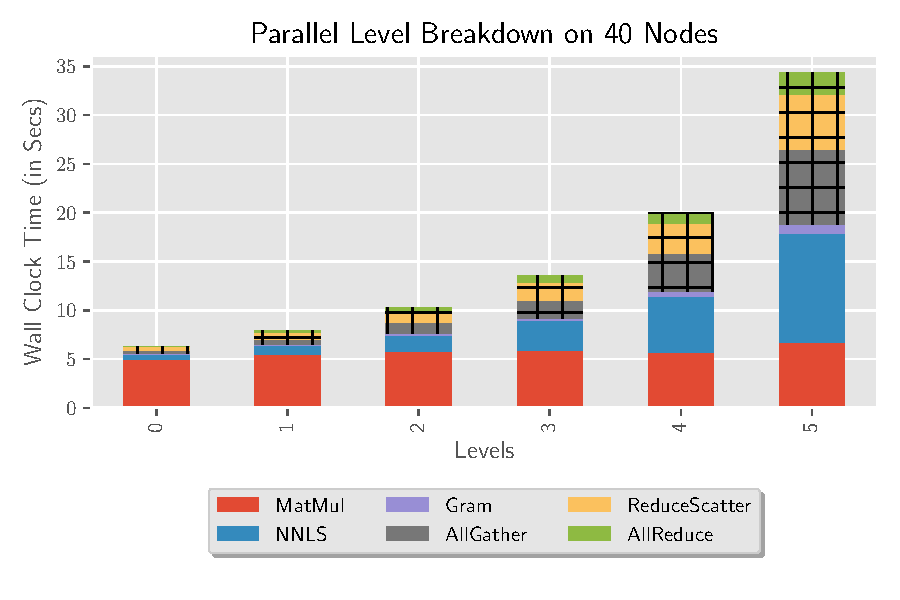
\includegraphics[height=2in, width=\columnwidth]{plots/synthetic_parallel_level_breakdown.pdf}
\caption{Parallel Breakdown plot for levels 0 to 5 on 40 nodes. y-axis is absolute wall clock time in seconds}
\label{fig:parallellevelbreakdown}
\end{center}
\end{figure}


\begin{figure}
\begin{center}
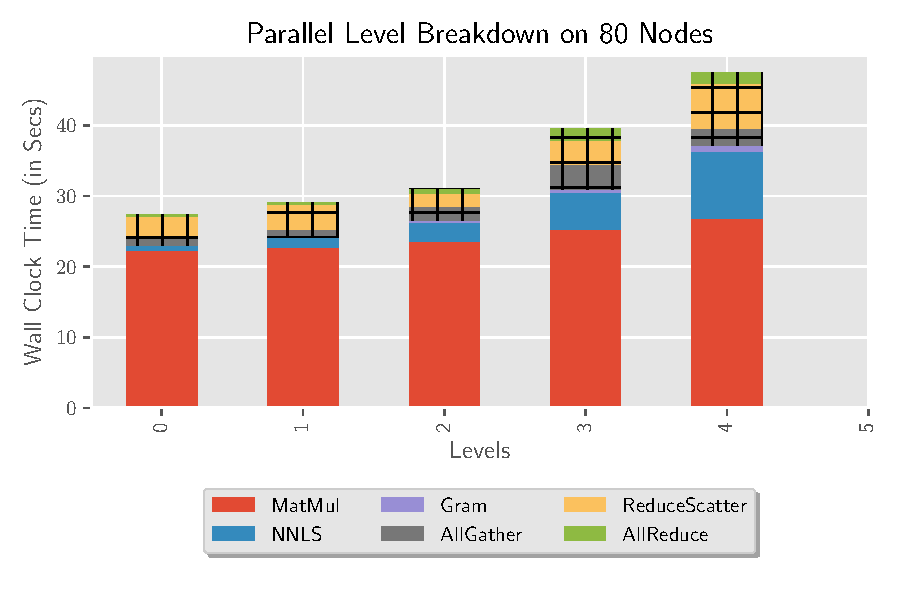
\includegraphics[height=2in, width=\columnwidth]{plots/realworld_parallel_level_breakdown.pdf}
\caption{Parallel Breakdown plot for levels 0 to 5 on 80 nodes. y-axis is absolute wall clock time in seconds}
\label{fig:rwparallellevelbreakdown}
\end{center}
\end{figure}


\subsection{DC Clustering Results}

\subsubsection{Hyperspectral Imaging}
\begin{figure}
% !TEX root = ../paper.tex

\resizebox{\columnwidth}{!}{
\begin{tikzpicture}
    \node[inner sep=0pt] (original) at (0,0)
        {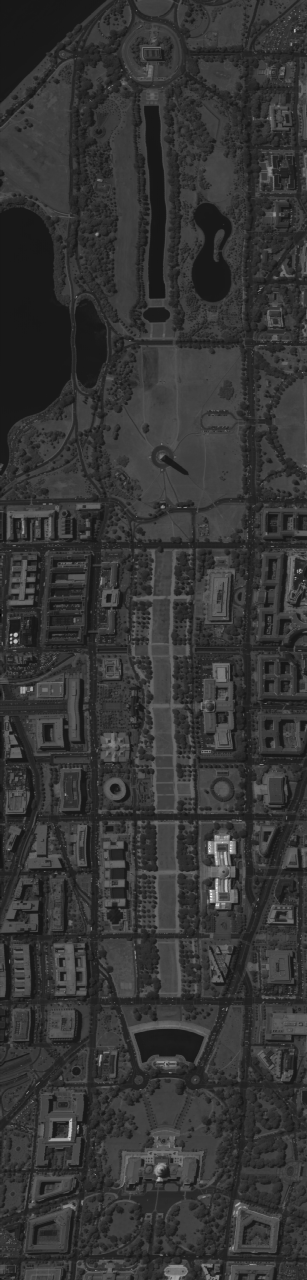
\includegraphics[width=0.8cm,height=3.2cm]{data/DC/0.png}};
        \draw[thick,->] (-0.4,0.8) .. controls (-3,0.8) .. (-3,-0.4);
        \node[inner sep=0pt] (1) at (-3,-2)
            {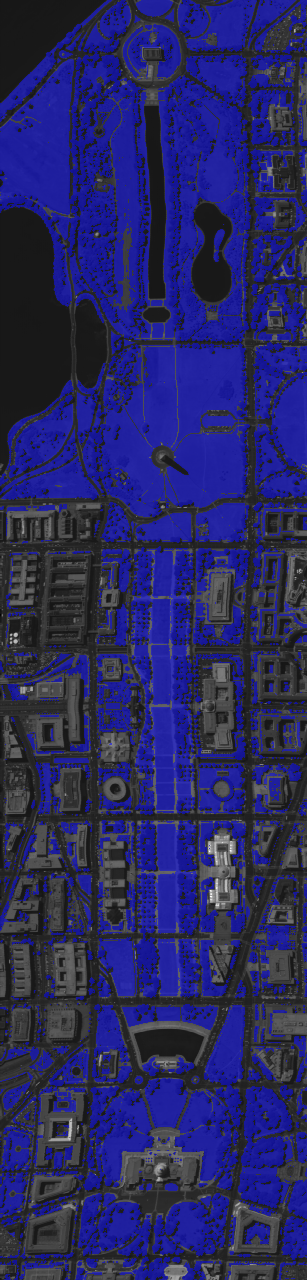
\includegraphics[width=0.8cm,height=3.2cm]{data/DC/1.png}};
            \draw[thick,->] (-2.6,-1.2) .. controls (-1.6,-1.2) .. (-1.6,-2.4);
            \node[inner sep=0pt] (3) at (-1.6,-4)
                {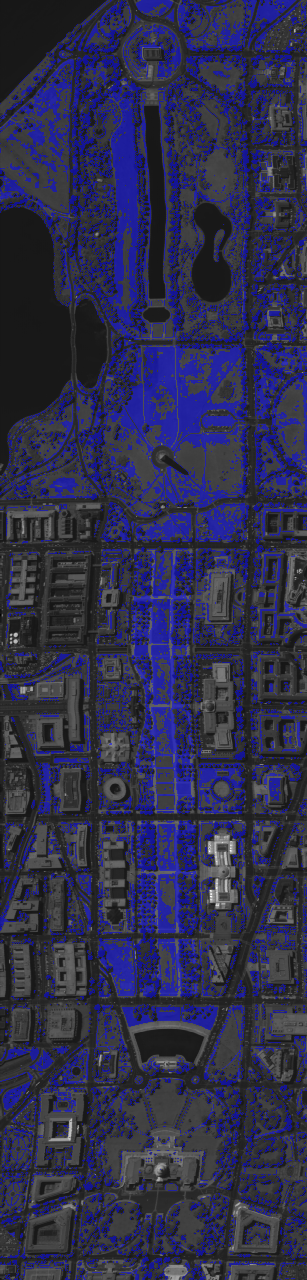
\includegraphics[width=0.8cm,height=3.2cm]{data/DC/3.png}};
                \draw[thick,->] (-2,-3.2) .. controls (-2.5,-3.2) .. (-2.5,-4.4);
                \node[inner sep=0pt] (7) at (-2.5,-6)
                    {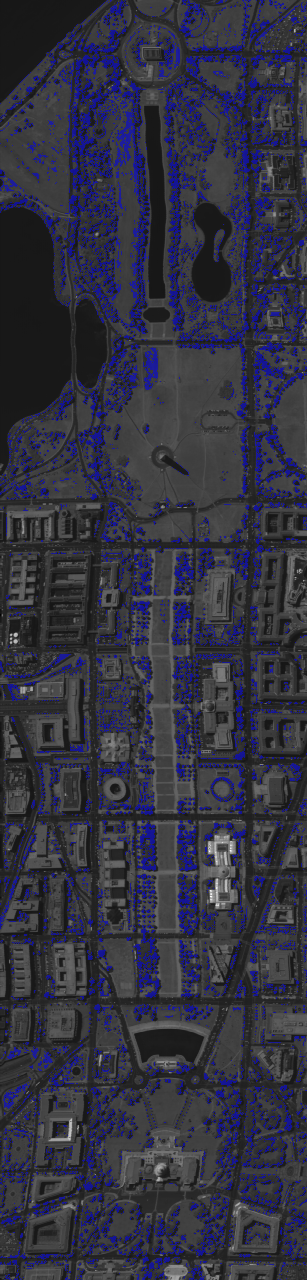
\includegraphics[width=0.8cm,height=3.2cm]{data/DC/7.png}};
                \draw[thick,->] (-1.2,-3.2) .. controls (-0.7,-3.2) .. (-0.7,-4.4);
                \node[inner sep=0pt] (8) at (-0.7,-6)
                    {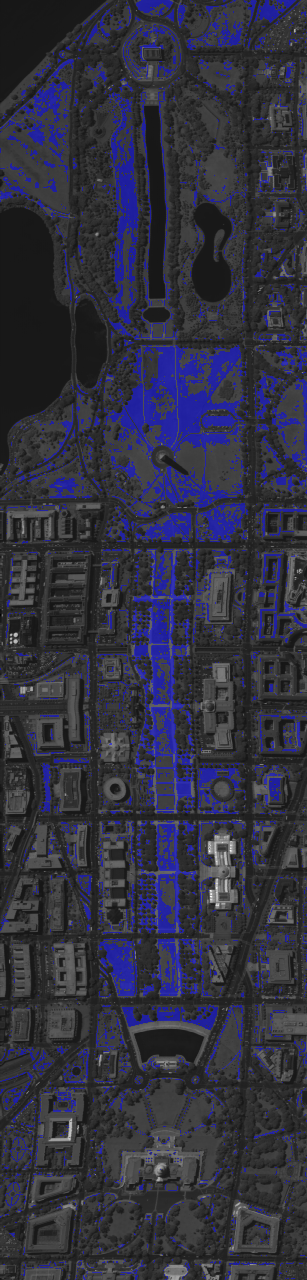
\includegraphics[width=0.8cm,height=3.2cm]{data/DC/8.png}};
            \draw[thick,->] (-3.4,-1.2) .. controls (-4.4,-1.2) .. (-4.4,-2.4);
            \node[inner sep=0pt] (4) at (-4.4,-4)
                {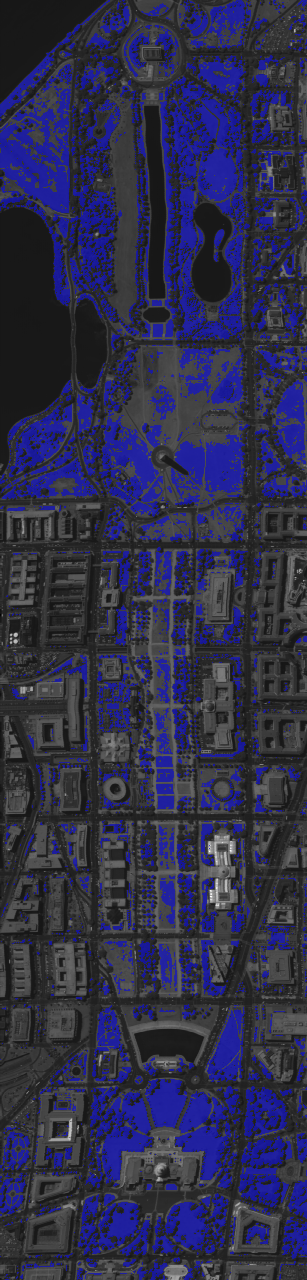
\includegraphics[width=0.8cm,height=3.2cm]{data/DC/4.png}};
        \draw[thick,->] (0.4,0.8) .. controls (3,0.8) .. (3,-0.4);
        \node[inner sep=0pt] (2) at (3,-2)
            {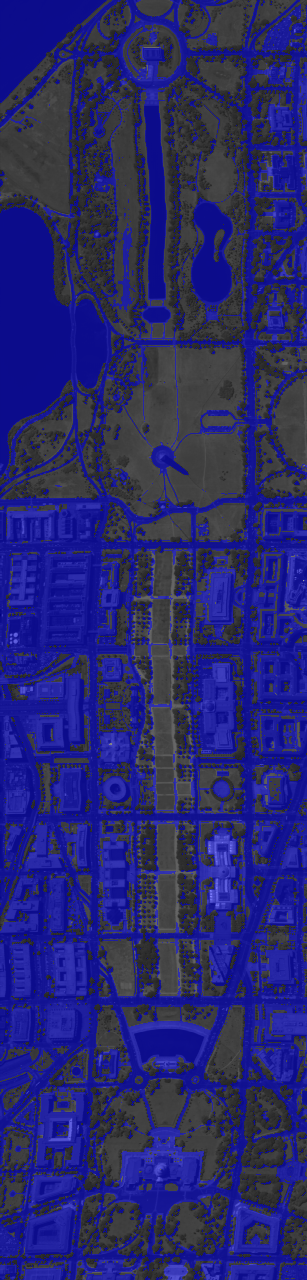
\includegraphics[width=0.8cm,height=3.2cm]{data/DC/2.png}};
            \draw[thick,->] (3.4,-1.2) .. controls (4.4,-1.2) .. (4.4,-2.4);
            \node[inner sep=0pt] (5) at (4.4,-4)
                {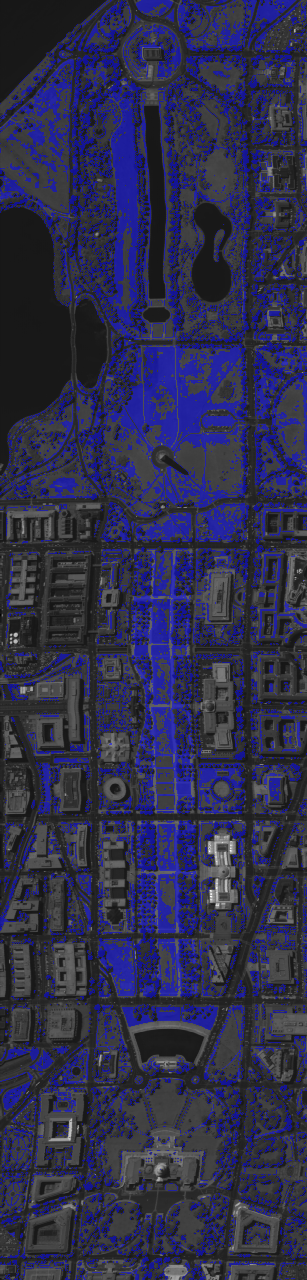
\includegraphics[width=0.8cm,height=3.2cm]{data/DC/3.png}};
            \draw[thick,->] (2.6,-1.2) .. controls (1.6,-1.2) .. (1.6,-2.4);
            \node[inner sep=0pt] (6) at (1.6,-4)
                {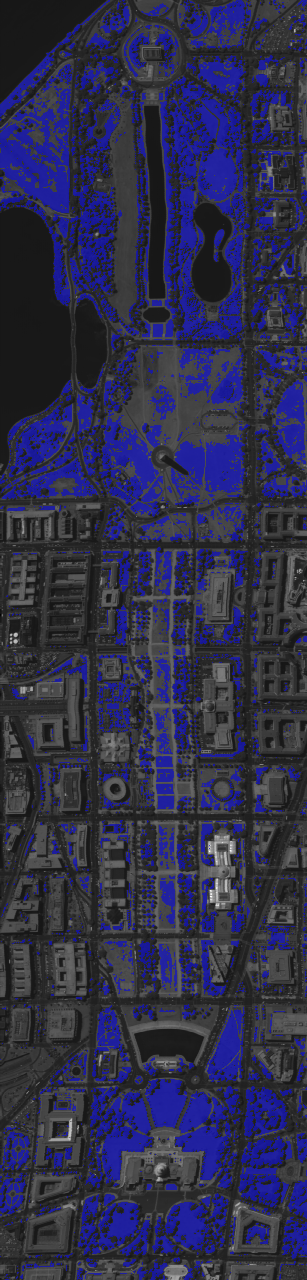
\includegraphics[width=0.8cm,height=3.2cm]{data/DC/4.png}};
                \draw[thick,->] (1.2,-3.2) .. controls (0.7,-3.2) .. (0.7,-4.4);
                \node[inner sep=0pt] (13) at (0.7,-6)
                    {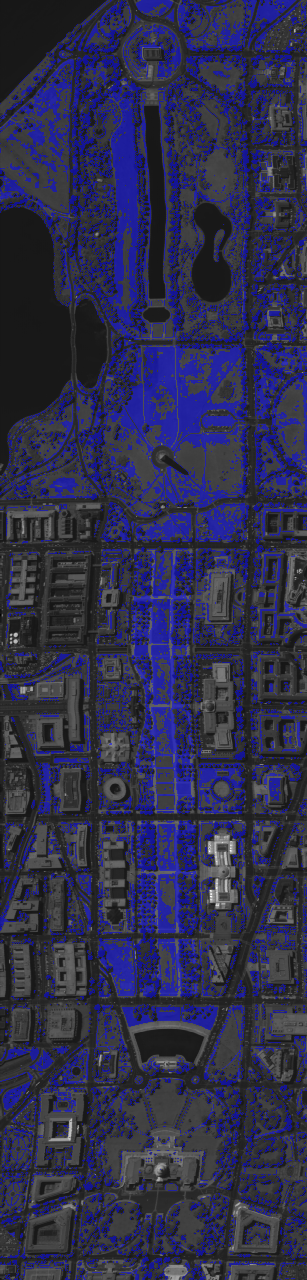
\includegraphics[width=0.8cm,height=3.2cm]{data/DC/3.png}};
                    \draw[thick,->] (2,-3.2) .. controls (2.5,-3.2) .. (2.5,-4.4);
                \node[inner sep=0pt] (14) at (2.5,-6)
                    {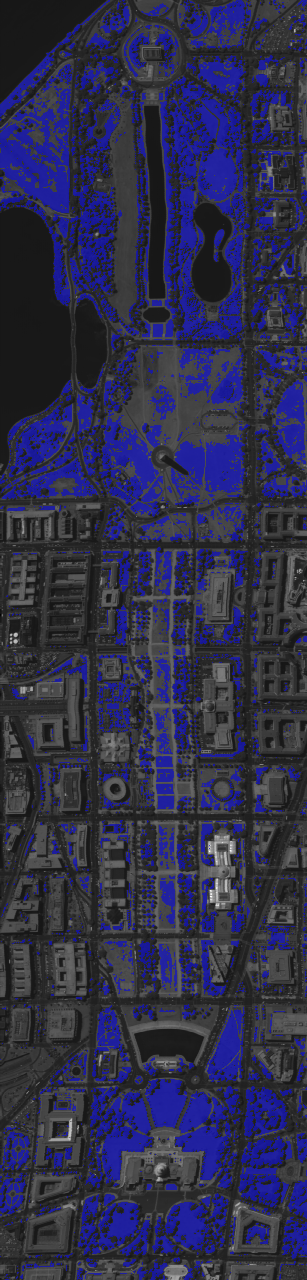
\includegraphics[width=0.8cm,height=3.2cm]{data/DC/4.png}};
\end{tikzpicture}
}
\caption{Hierarchical Cluster from DC Mall Image}
\label{fig:dc}
\end{figure}


\section{Conclusion}

\begin{itemize}
	\item consider sparse case
	\item consider parallelizing across tree
	\item consider redistribution for 2D
\end{itemize}

\section*{Acknowledgment}

The authors would like to thank Simin Ma for contributions to the algorithmic analysis and John Farrell for his contributions to the implementation of the parallel algorithm.

\bibliography{paper}
\bibliographystyle{plainurl}

\end{document}
